\section{Motion Planning Using Point Mass} \label{sec:motion_planning_using_point_mass}

In Section \ref{subsec:point_mass_model}, we introduced the point mass model with global coordinates and no orientation.
We now extend this model to the Frenet frame, which allows for a more structured approach to motion planning along a predefined road.
The idea and the equations are based on the work of Eilbrecht et al.
\cite{eilbrecht_challenges_2020}.

To achieve this, we first define the curvature of the reference path, which quantifies the rate of change of the tangent angle with respect to arc length:
\begin{equation}
	C := \frac{d\theta}{ds}.
\end{equation}
Additionally, let $\psi$ be the orientation of the vehicle, and define the alignment error $\xi$ as the difference between the vehicle's orientation and the reference path's tangent angle:
\begin{equation}
	\xi := \psi - \theta.
\end{equation}
This alignment error measures the deviation of the vehicle's heading from the reference path.

Using these definitions, along with established kinematic relationships and coordinate frame transformations \cite{eilbrecht_challenges_2020}, we can
systematically derive the motion dynamics in the Frenet frame.
These equations describe how the vehicle's velocity components in the body-fixed frame relate to changes in Frenet frame coordinates.

The first-order derivatives are given by:
\begin{align}
	\dot{s}(1 - nC(s)) & = v_x\cos{\xi} - v_y\sin{\xi}, \label{eq:first_derivative_long} \\
	\dot{n}            & = v_x\sin{\xi} + v_y\cos{\xi}. \label{eq:first_derivative_lat}
\end{align}

These equations describe the evolution of the vehicle's longitudinal and lateral positions in the Frenet frame.
The presence of the curvature term $C(s)$ ensures that the equations correctly account for the curvature of the reference path.

For the second derivatives, we obtain:
\begin{align}
	a_{x,tn} & = (a_x - v_y\dot{\psi})\cos{\xi} - (a_y + v_x\dot{\psi})\sin{\xi}, \label{eq:second_derivative_long} \\
	a_{y,tn} & = (a_x - v_y\dot{\psi})\sin{\xi} + (a_y + v_x\dot{\psi})\cos{\xi}. \label{eq:second_derivative_lat}
\end{align}

where the transformed acceleration terms in the Frenet frame are given by:
\begin{align}
	a_{x,tn} & := \ddot{s}(1 - nC(s)) - 2\dot{n}
	C(s)\dot{s} - nC'(s)\dot{s}^2, \label{def:axtn} \\ a_{y,tn} & := \ddot{n} + C(s)\dot{s}^2(1 - nC(s)).
	   \label{def:aytn}
\end{align}

In subsequent sections, we will leverage these equations to develop motion planning strategies that optimize trajectory feasibility and control
performance.

\subsection{Conversion of Global Cartesian Coordinates to Frenet Frame Coordinates} \label{subsec:pm_conversion_of_cartesian_to_frenet}

We now define the state variables $x_0$, representing the vehicle's position, orientation, and velocities in the Frenet frame, along with the control inputs $u_0$ for our point mass model in the Frenet frame:

\begin{equation}
	x_0 = \begin{bmatrix}
		s       &
		n       &
		\xi     &
		\dot{s} &
		\dot{n} &
		\dot{\psi}
	\end{bmatrix}^T
\end{equation}

The state vector consists of the Frenet frame coordinates that define the vehicle's location, the alignment error representing the deviation of the
vehicle's orientation from the reference path, and the first-order time derivatives of these quantities, which capture the vehicle's velocity
components.

We define the following three control inputs:

\begin{equation}
	u_0 = \begin{bmatrix}
		a_{x} &
		a_{y} &
		a_\psi
	\end{bmatrix}^T
\end{equation}

Using the previously derived equations, we can formulate the model dynamics in the Frenet frame as:

\begin{equation}
	\label{eq:frenet_frame_pm_dynamics_0}
	f_0(x_0, u_0) = \begin{bmatrix}
		\dot{s}                                  \\
		\dot{n}                                  \\
		\dot{\psi} - C(s)\dot{s}                 \\
		\frac{a_{x,tn} + 2\dot{n}
		C(s)\dot{s}+nC'(s)\dot{s}^2} { 1-nC(s) } \\ a_{y,tn} - C(s)\dot{s}^2(1-nC(s)) \\ a_\psi\end{bmatrix} \end{equation}

With this
formulation, we are now able to model vehicle motion in the Frenet frame along a predefined road.
However, the inclusion of curvature terms introduces non-convexity into the system dynamics.
In the following section, we will explore methods to address this challenge and develop techniques to handle the resulting non-convex constraints
effectively.

\subsection{System Linearization} \label{subsec:constraints}

First, we decouple the input.
By examining the dynamics equations \eqref{eq:frenet_frame_pm_dynamics_0} and substituting the equations \eqref{def:axtn} and \eqref{def:aytn}, we
observe that the last two entries both contain the control inputs $a_x$ and $a_y$.
We proceed by making the following assumption:

\subsubsection{Assumption: Alignment Error}

Orientation of the vehicle $\psi$ equals the angle of the road $\theta$:
\begin{equation}
	\xi = \psi - \theta = 0
\end{equation}
which directly implies the following three points, which will help us in further steps:
\begin{align}
	[a_x, a_y] & = [a_{x,tn}, a_{y,tn}]                                                \\
	\dot{\psi} & = \dot{\theta} = \frac{d\theta}{ds} \cdot \frac{ds}{dt} = C(s)\dot{s} \\
	a_\psi     & = \ddot{\psi} = \ddot{\theta} = C'(s) \dot{s}^2 + C(s)\ddot{s}
\end{align}

At first glance, it seems like we are removing the orientation from our model, but we actually just force the vehicle to always be aligned with the
road.
And since we allow lateral acceleration of the vehicle, it is not fixed to a constant offset to the reference path and can still move left or right.

With this assumption we end up with dynamics equation, which are affine linear in $a_{x,tn}$ and $a_{y,tn}$.
This allows us to introduce artificial control inputs to linearize the dynamics.

\begin{equation}
	\label{eq:artificial_controls}
	\tilde{u} := \begin{bmatrix}
		u_t \\
		u_n
	\end{bmatrix} := \begin{bmatrix}
		\frac{a_{x,tn} + 2\dot{n}
		C(s)\dot{s}+nC'(s)\dot{s}^2} { 1-nC(s) } \\ a_{y,tn} - C(s)\dot{s}^2(1-nC(s))\end{bmatrix} \end{equation}

This procedure is
called Feedback Linearization and described in depth by \cite{khalil_nonlinear_2002}.
We want to shortly introduce the topic.

\subsubsection{Feedback Linearization}

Feedback linearization is a nonlinear control technique that transforms a nonlinear system into an equivalent linear system by means of a suitable
change of variables and an appropriate state-feedback law.
This approach allows one to apply classical linear control design methods to inherently nonlinear systems.

Consider a general nonlinear system of the form:
\begin{equation}
	\dot{x} = f(x) + G(x)\,u,
\end{equation}
where
\begin{itemize}
	\item $x \in \mathbb{R}^n$ is the state vector,
	\item $f(x)$ represents the system's dynamics,
	\item $G(x)$ is the input matrix,
	\item $u \in \mathbb{R}^m$ is the control input vector.
\end{itemize}

For feedback linearization, we typically assume the system is \emph{fully actuated}, which requires that \[ \text{rank}\bigl(G(x)\bigr) = n, \] i.e.,
$G(x)$ must be invertible for all $x$ in the region of interest.
This condition ensures that the control input $u$ directly influences every component of the state vector.

If $G(x)$ is invertible, then we can solve for the control input $u$ in terms of the state $x$, its dynamics, and a new artificial control input $v$.
Specifically,
\begin{equation}
	u = G(x)^{-1}\,\bigl[v - f(x)\bigr].
\end{equation}
By choosing $u$ in this way, the nonlinear dynamics $f(x)$ are effectively canceled, leaving the new input $v$ to be designed (using standard linear
control techniques) to achieve the desired closed-loop behavior.

\subsubsection{Resulting Simplified Model}

Since the orientation is fixed, we can remove it from the state variables, and we end up with the following state variables.
\[
	x_1 = \begin{bmatrix} s, & n, & \dot{s}, & \dot{n} \end{bmatrix}^T
\]
We use the new defined artificial controls inputs, for controlling the system.
\[
	\tilde{u} = \begin{bmatrix} u_t, & u_n \end{bmatrix}^T
\]
The dynamics are given by:
\begin{equation}
	f_1(x_1, \tilde{u}) = \begin{bmatrix}
		\dot{s} \\
		\dot{n} \\
		u_t     \\
		u_n     \\
	\end{bmatrix}
	\label{eq:pm_final_dynamics}
\end{equation}

\subsubsection{Constraints}

We have addressed the dynamics constraints of our discrete-time optimal trajectory planning problem \eqref{eq:discrete_dynamics}.
Next, we will define the coupling constraints on the state variables and control inputs, discuss the arising challenges, and explore potential
solutions.

First, let's examine the vehicle constraints \cite{eilbrecht_challenges_2020}.
Let $\square$ represent one of the variables used in trajectory planning.
The upper bound is denoted by $\overline{\square}$, and the lower bound by $\underline{\square}$, both of which remain constant during planning.

Constraints on the velocity are defined in a body-fixed manner, with upper and lower bounds, using the following annotations.

\begin{align}
	\underline{v_x} \leq v_x \leq \overline{v_x} \\
	\underline{v_y} \leq v_y \leq \overline{v_y}
\end{align}

We can easily apply \eqref{eq:first_derivative_lat} and \eqref{eq:first_derivative_long} to get resulting constraints on our state variables.
The equations reduce together with $\xi = 0$ to:

\begin{align}
	\underline{v_x}  \leq  \dot{s}(1-nC(s))  \leq  \overline{v_x} \\
	\underline{v_y}  \leq  \dot{n}           \leq  \overline{v_y}
\end{align}

For the acceleration two types of constraints are usually defined, the first one which constrains the relations of the longitudinal and lateral acceleration as:
\begin{equation}
	a_x^2 + a_y^2 \leq c
\end{equation}
for some constant radius $c\in \mathbb{R}^+$, the second similar to the velocity as follows:
\begin{align}
	\underline{a_x} \leq a_x \leq \overline{a_x} \\
	\underline{a_y} \leq a_y \leq \overline{a_y}
\end{align}

Using our derived equations, we can define a mapping from the model's state variables and artificial control inputs to the body-fixed accelerations.

\begin{equation}
	g(x_1, \tilde{u}) :=
	\begin{bmatrix}
		(1 - nC(s)) u_t - (2\dot{n}C(s)\dot{s} + nC' \dot{s}^2) \\
		u_n + C(s) \dot{s}^2 (1 - nC(s))
	\end{bmatrix}  = \begin{bmatrix}
		a_x \\
		a_y
	\end{bmatrix}
	\label{def:g}
\end{equation}
Combining the vehicle constraints derived from the body-fixed frame and the straightforward constraints given by the road, we can define our coupling constraint set $\mathcal{C}$ as:
\begin{equation}
	\mathcal{C} := \left\{
	\begin{bmatrix} x_1 \\ \tilde{u} \end{bmatrix} \; \middle|\;
	\begin{aligned}
		 & \underline{s} \leq s \leq \overline{s},                                     \\
		 & \underline{n}(s) \leq n \leq \overline{n}(s),                               \\
		 & \underline{v_x}  \leq  \dot{s}(1-nC(s))  \leq  \overline{v_x}               \\
		 & \underline{v_y} \leq \dot{n} \leq \overline{v_y}                            \\
		 & \underline{\dot{\psi}} \leq C(s) \dot{s} \leq \overline{\dot{\psi}},        \\
		 & \underline{a_{\psi}} \leq C' \dot{s}^2 + C(s) u_t \leq \overline{a_{\psi}}, \\
		 & \begin{bmatrix}
			   \underline{a_x} \\ \underline{a_y}
		   \end{bmatrix} \leq g(x_1, \tilde{u}) \leq \begin{bmatrix}
			                                             \overline{a_x} \\\overline{a_y}
		                                             \end{bmatrix}    \\
		 & ||g(x_1, \tilde{u})||^2 \leq c
	\end{aligned}
	\right\}
\end{equation}

This set is highly non-convex, and we now face the challenge of transforming these constraints into a convex form.
We will address this by finding an inner polytope of the set $\mathcal{C}$ as follows.

\subsubsection{Problem Definition: Finding an Inner Polytope}
\label{problem:inner_polytope}
Given set $\mathcal{C}$ over the state variables $x_1$ and control inputs $\tilde{u}$, find $\underline{\mathcal{C}}$, such that:
\begin{equation}
	\underline{\mathcal{C}} = \left\{ \begin{bmatrix}
		x_1 \\ \tilde{u} \end{bmatrix} \; \middle|\;
	N \begin{bmatrix}
		x_1 \\ \tilde{u} \end{bmatrix} \leq b
	\right\} \subseteq \mathcal{C}
\end{equation}

We will demonstrate two methods to achieve this goal, both aiming to accomplish the following:

We want to find the set $\tilde{\underline{\mathcal{C}}}$ over the variables $\dot{s}$ and $\tilde{u}$, such that:

\begin{equation}
	\tilde{\underline{\mathcal{C}}} =
	\left\{ \;
	\begin{bmatrix}
		\dot{s} \\
		u_t     \\
		u_n
	\end{bmatrix}
	\middle|\;
	\begin{bmatrix}
		x_1 \\ \tilde{u}
	\end{bmatrix} \in \mathcal{C}, \text{for all } \begin{bmatrix}
		s \\
		n \\
		\dot{n}
	\end{bmatrix} \in \begin{bmatrix}
		\underline{s}, \overline{s} \\
		\underline{n}, \overline{n} \\
		\underline{\dot{n}},  \overline{\dot{n}}
	\end{bmatrix}
	\right\}
\end{equation}

Specifically, we aim to find a set of linear inequalities, each representing a half-space, such that the intersection of these half-spaces forms the
set $\tilde{\underline{\mathcal{C}}}$.
The following condition should then be satisfied:

\begin{equation}
	\label{eq:forall_formula}
	\begin{bmatrix}
		\dot{s} \\
		u_t     \\
		u_n
	\end{bmatrix} \in \tilde{\underline{\mathcal{C}}}
	\implies
	\forall  \begin{bmatrix}
		s \\
		n \\
		\dot{n}
	\end{bmatrix} \in \begin{bmatrix}
		\underline{s}, \overline{s} \\
		\underline{n}, \overline{n} \\
		\underline{\dot{n}},  \overline{\dot{n}}
	\end{bmatrix}: \quad
	\begin{aligned}
		 & (\underline{v_x}  \leq  \dot{s}(1-nC(s))  \leq  \overline{v_x}             & \land \\
		 & \underline{\dot{\psi}} \leq C(s) \dot{s} \leq \overline{\dot{\psi}}        & \land \\
		 & \underline{a_{\psi}} \leq C' \dot{s}^2 + C(s) u_t \leq \overline{a_{\psi}} & \land \\
		 & \begin{bmatrix}
			   \underline{a_x} \\ \underline{a_y}
		   \end{bmatrix} \leq g(x_1, \tilde{u}) \leq \begin{bmatrix}
			                                             \overline{a_x} \\\overline{a_y}
		                                             \end{bmatrix}                  & \land   \\
		 & ||g(x_1, \tilde{u})||^2 \leq c )
	\end{aligned}
\end{equation}

\subsection{Eliminating the For-All Operator} \label{subsec:eliminating_the_for_all_operator}

Solving the problem of finding an inner polytope of the set $\mathcal{C}$ requires addressing the universal quantifier in \eqref{eq:forall_formula}.
We will explore two methods to eliminate this operator and find a polytope that satisfies the constraints for all possible values of the state
variables $s$, $n$, and $\dot{n}$.

\subsubsection{Interval Fitting for State Variables and Control Inputs}

The first approach is computationally less expensive but results in a smaller feasible set.
Despite this, it performs remarkably well.
The idea is to find intervals for the variables of interest, namely $\dot{s}$, $u_t$, and $u_n$, such that for any values these variables may take
within those intervals, the implications from \eqref{eq:forall_formula} hold.
Each condition of these implications follows a specific pattern.
Let $x \in \{\dot{s}, u_t, u_n\}$ and $y$ be a vector containing the remaining variables that are part of the condition.
\begin{equation}
	\label{eq:cur_condition}
	c_{min} \leq f(x, y) \leq c_{max}
\end{equation}
where $x \in \mathbb{R}$, $y \in \mathbb{R}^n$, and $f: \mathbb{R}^{n+1} \to \mathbb{R}$, with constants $c_{min}, c_{max} \in \mathbb{R}$.
The variable $x$ is selected such that all other variables contained in $y$ are bounded.
Additionally, $x$ is chosen so that $f$ is affine in $x$, represented by:
\begin{equation}
	f(x, y) = a(y) x + b(y)
\end{equation}
where $a, b : \mathbb{R}^n \to \mathbb{R}$. Since $a$ and $b$ are continuous functions over a bounded domain $Y$, we can find bounds on $a(y)$ and $b(y)$:
\begin{equation}
	a_{min} \leq a(y) \leq a_{max}, \quad b_{min} \leq b(y) \leq b_{max}
\end{equation}
Our goal is to find an interval $[\underline{x}, \overline{x}]$ for $x$ such that
\begin{equation}
	x\in [\underline{x}, \overline{x}] \implies \forall y\in Y: c_{min} \leq f(x, y) \leq c_{max}
\end{equation}

We define $X := [\underline{x}, \overline{x}]$.
To calculate $X$, we perform a case distinction based on the possible signs of $a(y)$.
Let's start with

\textbf{1.
}
$a(y) > 0$:
We can subtract \eqref{eq:cur_condition} with $b(y)$ and divide by $a(y)$:
\[
	\frac{c_{min}-b(y)}{a(y)} \leq x \leq \frac{c_{max}-b(y)}{a(y)}
\]
Since we have to ensure the condition holds even in the worst case, $X$ is given by:
\[
	\underline{x} =
	\begin{cases}
		\begin{array}{ll}
			\frac{c_{min}-b_{min}}{a_{max}}, & \text{if } c_{min}-b_{min} < 0 \\[10pt]
			\frac{c_{min}-b_{min}}{a_{min}}, & \text{otherwise}
		\end{array}
	\end{cases}
\]
\[
	\overline{x} =
	\begin{cases}
		\begin{array}{ll}
			\frac{c_{max}-b_{max}}{a_{min}}, & \text{if } c_{max}-b_{max} < 0 \\[10pt]
			\frac{c_{max}-b_{max}}{a_{max}}, & \text{otherwise}
		\end{array}
	\end{cases}
\]

\textbf{2.}
$a(y) \geq 0$:
Since $a(y) = 0$ for some $y\in Y$, we have to test if this condition holds:
\[
	c_{min} \leq b_{min} \text{ and } b_{max} \leq c_{max}
\]
If this condition does not hold, then $X=\emptyset$.
Otherwise, we exclude all $y \in Y$ for which $a(y)=0$ and proceed to the first case.

\textbf{3.}
$a(y) < 0$:
We can again subtract $b(y)$ from \eqref{eq:cur_condition} and divide by $a(y)$, but this time the direction of the inequalities changes:
\[
	\frac{c_{max}-b(y)}{a(y)} \leq x \leq \frac{c_{min}-b(y)}{a(y)}
\]
and by looking at the worst cases of the lower and upper bound, we can calculate $X$:
\[
	\underline{x} =
	\begin{cases}
		\begin{array}{ll}
			\frac{c_{max}-b_{max}}{a_{max}}, & \text{if } c_{max}-b_{max} < 0 \\[10pt]
			\frac{c_{max}-b_{max}}{a_{min}}, & \text{otherwise}
		\end{array}
	\end{cases}
\]
\[
	\overline{x} =
	\begin{cases}
		\begin{array}{ll}
			\frac{c_{min}-b_{min}}{a_{min}}, & \text{if } c_{min}-b_{min} < 0 \\[10pt]
			\frac{c_{min}-b_{min}}{a_{max}}, & \text{otherwise}
		\end{array}
	\end{cases}
\]

\textbf{4.}
$a(y) \leq 0$:
Similar to the second case, we need to check if $c_{min} \leq b_{min}$ and $b_{max} \leq c_{max}$ hold.
If not, set $X=\emptyset$.
Otherwise, ignore the values where $a(y)$ equals zero and proceed to the third case.

\textbf{5.}
We have so far considered all the cases where $a(y)$ cannot take both positive and negative values.
We now consider the last case, where $a_{min} < 0$ and $a_{max} > 0$.
Since $a(y) = 0$ for some values, we first check if $c_{min} \leq b_{min}$ and $b_{max} \leq c_{max}$.
If this condition does not hold, we set $X = \emptyset$.
Otherwise, $X$ is given by:

\[ \underline{x} = \max \left\{ \frac{c_{min} - b_{min}}{a_{max}}, \frac{c_{max} - b_{max}}{a_{min}}
	\right\} \]

\[ \overline{x} = \min \left\{ \frac{c_{max} - b_{max}}{a_{max}}, \frac{c_{min} - b_{min}}{a_{min}} \right\} \]

If we end up with $x_{max} < x_{min}$, set $X=\emptyset$.

All of this applies nicely to our scenario, as we can systematically apply these rules to each constraint step by step.
The resulting polytope, based on the interval approach, is box-shaped.
This shape further reduces our set of possible state variables and control inputs.

\subsubsection{Cylindrical Algebraic Decomposition}

The second approach is to use Cylindrical Algebraic Decomposition (CAD) to find the inner polytope.
This method is computationally more expensive but provides a more accurate result.
The idea is to find an equivalent formula without quantifiers for a given formula containing quantifiers.
This can be done using CAD.

CAD is a method used in computer algebra for solving systems of polynomial equations and inequalities.
Given a set of polynomial equations and inequalities, CAD decomposes the space into a finite number of cylindrical cells.
Each cell is described by a sequence of polynomial inequalities and has a constant truth value over the input set of polynomial equations and
inequalities.
This way, one only needs to pick one point from each cell to check the truth value of the input set.
The number of cells grows doubly exponentially with the number of variables in the input set.
Several implementations of CAD exist.

We will illustrate how the algorithm works, but it is beyond the scope of this work to explain the implementations in detail.
Instead, we provide a basic example to illustrate the algorithm without delving into the details.
You can find more information in the literature \cite{caviness_quantifier_1998, england_cylindrical_2020}.

\subsubsection{Example}
To illustrate the process of eliminating $\forall$ quantifiers, consider the following problem:

\[ \forall x, x^2 + bx + 1 \geq 0
\]

Since quantifier elimination is typically performed on existential quantifiers, we first solve the problem for:

\[ \exists x, x^2 + bx + 1 < 0 \]

Once we have the solution for this problem, we can take the complement over
$\mathbb{R}$ to obtain the solution for the original problem.
We start by applying CAD to the polynomial $x^2 + bx + 1$, which results in 7 cells, as illustrated in Figure \ref{fig:example_cells}.
Most of the cells are open, and if the edge of the cell is part of it, it is depicted with the same color but dashed.

\begin{figure}[h]
	\centering
	\definecolor{redviolet}{rgb}{0.78, 0.08, 0.52}
	\begin{tikzpicture}
		\begin{axis}[
				xlabel={$b$},
				ylabel={$x$},
				axis lines=middle,
				enlargelimits=true,
				legend pos=north west,
			]

			% Define the boundaries as paths
			\addplot [name path=RightUpper, domain=2:5, samples=100, thick, redviolet!30, dashed] {-(x/2) + 1/2 * sqrt(-4 + x^2)};
			\addplot [name path=RightLower, domain=2:5, samples=100, thick, teal!30, dashed] {-(x/2) - 1/2 * sqrt(-4 + x^2)};
			\addplot [name path=LeftUpper, domain=-5:-2, samples=100, thick,blue!30, dashed] {-(x/2) + 1/2 * sqrt(-4 + x^2)};
			\addplot [name path=LeftLower, domain=-5:-2, samples=100, thick,cyan!30, dashed] {-(x/2) - 1/2 * sqrt(-4 + x^2)};

			% Define vertical lines as paths but make them invisible
			\addplot [name path=lineInnerRight,dashed, thick,  red!30] coordinates {(2,-5) (2,5)};
			\addplot [name path=lineInnerLeft, dashed, thick, red!30] coordinates {(-2,-5) (-2,5)};

			% Define horizontal boundaries as paths but make them invisible
			\addplot [name path=lineUpperLeft, draw=none] coordinates {(-5,5) (-2,5)};
			\addplot [name path=lineUpperRight, draw=none] coordinates {(2,5) (5,5)};
			\addplot [name path=lineLowerLeft, draw=none] coordinates {(-5,-5) (-2,-5)};
			\addplot [name path=lineLowerRight, draw=none] coordinates {(2,-5) (5,-5)};

			% Region 1: b>2, x >= -(b/2) + 1/2 sqrt(-4 + b^2)
			\addplot [fill=redviolet!30, opacity=0.5] fill between[of=RightUpper and lineUpperRight];

			% % Region 2: b>2, x <= -(b/2) - 1/2 sqrt(-4 + b^2)
			\addplot [fill=teal!30, opacity=0.5] fill between[of=RightLower and lineLowerRight];

			% % Region 3: b<-2, x >= -(b/2) + 1/2 sqrt(-4 + b^2)
			\addplot [fill=blue!30, opacity=0.5] fill between[of=LeftUpper and lineUpperLeft];

			% % Region 4: b<-2, x <= -(b/2) - 1/2 sqrt(-4 + b^2)
			\addplot [fill=cyan!30, opacity=0.5] fill between[of=LeftLower and lineLowerLeft];

			% % Region 5: -2 ≤ b ≤ 2 (rectangle covering all x values)
			\addplot [fill=red!30, opacity=0.5] fill between[of=lineInnerLeft and lineInnerRight];

			% % Region 6: b>2, x > -(b/2) - 1/2 Sqrt[-4+b^2], x < -(b/2) + 1/2 Sqrt[-4+b^2]
			\addplot [fill=cyan!30, opacity=0.3] fill between[of=RightUpper and RightLower];

			% % Region 7: b<-2, x > -(b/2) - 1/2 Sqrt[-4+b^2], x < -(b/2) + 1/2 Sqrt[-4+b^2]
			\addplot [fill=gray!30, opacity=0.3] fill between[of=LeftUpper and LeftLower];

		\end{axis}
	\end{tikzpicture}
	\caption{Illustrating the cells with shaded regions.}
	\label{fig:example_cells}
\end{figure}
We now need to check the truth value of the polynomial inequality $x^2 + bx + 1 < 0$ for each cell by picking a random sample and evaluating the
inequality.
The cells where the inequality holds true are colored in green and then projected onto the $b$-axis.
The resulting intervals are the solution to the existential quantifier elimination, which is $(-\infty, -2) \cup (2, \infty)$.
As an input to the algorithm, one must define an order of precedence for the variables.
In its first phase, the algorithm projects the space iteratively from $\mathbb{R}^n$ to $\mathbb{R}^{n-1}$ until it reaches $\mathbb{R}^1$.
This is done by removing one of the remaining variables in each iteration, starting with the last in the order of precedence.
Therefore, if $b$ is defined as the first variable, the sets of polynomial inequalities for each cell will always contain an interval for $b$, which
corresponds to the projection on the axis.
This allows us to directly read the resulting intervals, which is shown in Figure \ref{fig:remaining_cells}.

\begin{figure}[h]
	\centering
	\begin{tikzpicture}
		\begin{axis}[
				xlabel={$b$},
				ylabel={$x$},
				axis lines=middle,
				enlargelimits=true,
				legend pos=north west,
			]

			% Define the boundaries as paths
			\addplot [name path=RightUpper, domain=2:5, samples=100, thick, black!30, dashed] {-(x/2) + 1/2 * sqrt(-4 + x^2)};
			\addplot [name path=RightLower, domain=2:5, samples=100, thick, black!30, dashed] {-(x/2) - 1/2 * sqrt(-4 + x^2)};
			\addplot [name path=LeftUpper, domain=-5:-2, samples=100, thick,black!30, dashed] {-(x/2) + 1/2 * sqrt(-4 + x^2)};
			\addplot [name path=LeftLower, domain=-5:-2, samples=100, thick,black!30, dashed] {-(x/2) - 1/2 * sqrt(-4 + x^2)};

			% Define vertical lines as paths but make them invisible
			\addplot [name path=lineInnerRight,dashed, thick,  draw=none] coordinates {(2,-5) (2,5)};
			\addplot [name path=lineInnerLeft, dashed, thick, draw=none] coordinates {(-2,-5) (-2,5)};

			% Define horizontal boundaries as paths but make them invisible
			\addplot [name path=lineUpperLeft, draw=none] coordinates {(-5,5) (-2,5)};
			\addplot [name path=lineUpperRight, draw=none] coordinates {(2,5) (5,5)};
			\addplot [name path=lineLowerLeft, draw=none] coordinates {(-5,-5) (-2,-5)};
			\addplot [name path=lineLowerRight, draw=none] coordinates {(2,-5) (5,-5)};

			% % Region 6: b>2, x > -(b/2) - 1/2 Sqrt[-4+b^2], x < -(b/2) + 1/2 Sqrt[-4+b^2]
			\addplot [fill=green!30, opacity=0.3] fill between[of=RightUpper and RightLower];

			% % Region 7: b<-2, x > -(b/2) - 1/2 Sqrt[-4+b^2], x < -(b/2) + 1/2 Sqrt[-4+b^2]
			\addplot [fill=green!30, opacity=0.3] fill between[of=LeftUpper and LeftLower];

			\node[circle,draw,inner sep=1pt, green!60] (openCircleRight) at (axis cs:2,0) {};
			\draw[thick, green!60] (openCircleRight) -- (axis cs:5.5,0);
			\node[circle,draw,inner sep=1pt, green!60] (openCircleLeft) at (axis cs:-2,0) {};
			\draw[thick, green!60] (openCircleLeft) -- (axis cs:-5.5,0);
		\end{axis}
	\end{tikzpicture}
	\caption{Illustrating the remaining cells.}
	\label{fig:remaining_cells}
\end{figure}
Since $(-\infty, -2) \cup (2, \infty)$ is the solution for $\exists x, x^2 + bx + 1 < 0$, the solution for the original problem is obtained by taking
the complement of this set:

\[ \forall x, x^2 + bx + 1 \geq 0 \iff b \in [-2, 2] \]

Using this technique for
eliminating quantifiers from formulas, we can apply it to find an inner polytope.

\subsubsection{Comparison of Interval Fitting and CAD Approaches}

In our benchmarks, the first approach, despite its simplicity, performed remarkably well.
We used the following parameters for the benchmarks:
\begin{itemize}
	\item $C(s) \in \left[-\frac{1}{200}, 0\right]$, $s \in [0, 10]$, $n \in [0, 2]$
	\item $v_x \in [0, 10]$, $v_y \in [-2, 2]$, $a_x \in [-3, 6]$, $a_y \in [-4, 4]$
	\item $\dot{\psi} \in [-5, 5]$, $a_\psi \in [-2, 2]$
\end{itemize}

The results are shown in the following figures \ref{fig:qe-comparison}.

\begin{figure}[h]
	\centering
	% First image
	\begin{subfigure}[b]{0.32\textwidth}
		\centering
		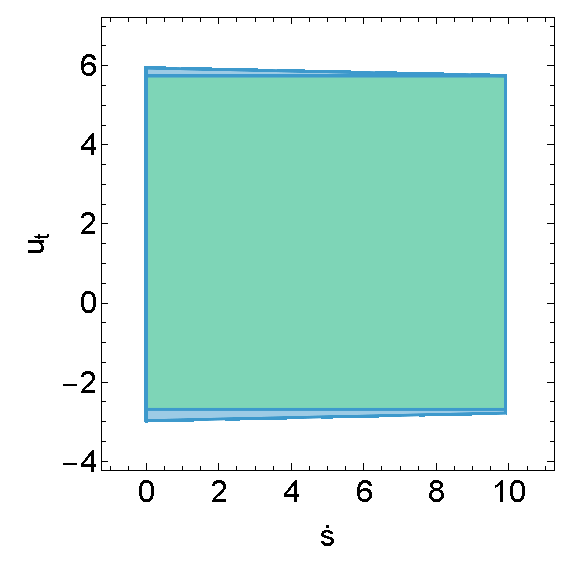
\includegraphics[width=\textwidth]{figures/inner_polytope/region_x3u1_plot_gr1.eps}
	\end{subfigure}
	% Second image
	\begin{subfigure}[b]{0.32\textwidth}
		\centering
		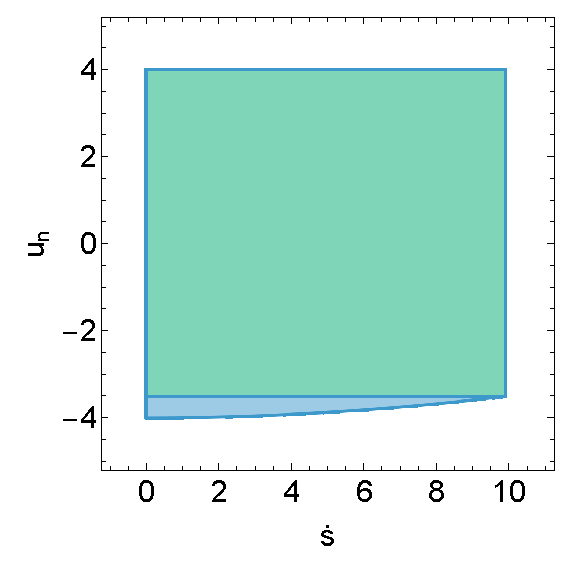
\includegraphics[width=\textwidth]{figures/inner_polytope/region_x3u2_plot_gr1.eps}
	\end{subfigure}
	% Third image
	\begin{subfigure}[b]{0.32\textwidth}
		\centering
		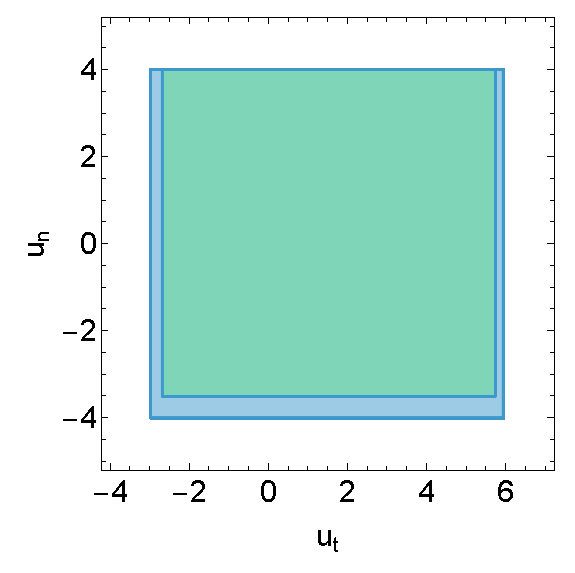
\includegraphics[width=\textwidth]{figures/inner_polytope/region_u1u2_plot_gr1.eps}
	\end{subfigure}
	\caption{In Green our first approach and in Blue using CAD.}
	\label{fig:qe-comparison}
\end{figure}

In conclusion, eliminating the quantifiers with the first approach leads to a near-optimal result, comparable to the one achieved using the second
approach with CAD.
However, using CAD has a significant downside that we have not yet mentioned.
It is not guaranteed that the resulting formula is convex.
Typically, you will encounter disjunctions of polynomial inequalities, which cannot be handled by a convex solver without resorting to integer
programming or an equivalent approach.
It is also not guaranteed that each polynomial inequality follows the DCP rules, even if the set described by the resulting formula is convex.
Additional techniques would be required to use the second approach for our planner.

In cases where the resulting set is convex, we used a sampling approach to obtain an inner approximation described by half-spaces.
This results in a sequence of linear constraints that all must be satisfied, thus losing a small proportion of the original set.
Consequently, the difference between our first approach and the second approach becomes even smaller.
Additionally, we end up with double or triple the number of constraints on each state variable and each control input, which may lead to slower
solver times.

Overall, while the CAD approach provides a more accurate result, the first approach offers a good balance between computational efficiency and
accuracy, making it a viable option for practical applications.

\subsubsection{Inner Polytope}

We have managed to construct a realistic model, which allows us to model any constraints arising either from the vehicle dynamics or the environment,
such that they are not only confirm with the DCP rules but also linear.

Our inner polytope from the problem \ref{problem:inner_polytope} is now given by:

\begin{equation}
	\label{eq:pm_coupling_constraints}
	\underline{\mathcal{C}} = \tilde{\underline{\mathcal{C}}} \times [\underline{s}, \overline{s}] \times [\underline{n}, \overline{n}] \times [\underline{\dot{n}}, \overline{\dot{n}}]
\end{equation}
with $\tilde{\underline{\mathcal{C}}}$ resulting from one of the presented $\forall$-elimination approach.

\subsubsection{Limitations and Outlook}

While the $\forall$-elimination approach provides a computationally efficient method to find intervals for the variables of interest, it can be quite restrictive for several reasons:

\begin{itemize}
	\item \textbf{Conservativeness:}
	      The approach tends to be conservative because it ensures that the constraints hold for all possible values within the intervals.
	      This often leads to smaller intervals, which may exclude feasible solutions that could be considered by less conservative methods.
	\item \textbf{Dependence on Affine Functions:}
	      The first method relies on the assumption that the function $f(x, y)$ is affine in $x$ and all variables in $y$ are bounded.
	      If this assumption does not hold, the approach may not be applicable.
\end{itemize}

Overall, while the $\forall$-elimination approach is useful for its simplicity and computational efficiency, it may lead to overly restrictive
solutions that do not fully exploit the feasible region.

Consider a scenario with a tight turn followed by a long straight road.
In such cases, the model will restrict $\dot{s}$ to an interval that is valid for both the tight turn and the straight road.
Consequently, the model will find a solution, but it will not be able to drive fast on the straight road, even though it is possible to drive faster
on the straight road than on the tight turn.

To address this issue, we can introduce segments of the road, one for the straight road and one for the tight turn.
We can independently construct the coupling constraints set for each segment.
However, this introduces a new problem: how to switch between the segments.
Our solution involves using the current vehicle velocity to predict when the vehicle will reach the end of the segment.
Knowing the vehicle's current position, velocity, and the distance to the end of the segment, we can calculate the time it will take to reach the
end.

Further, both approaches do not consider the possibility of achieving a larger feasible set by restricting $\dot{n}$ to a smaller interval.
The first approach handles the problem by using the bounds on $s$, $n$, and $\dot{n}$ to find the intervals for $\dot{s}$, which are then used for
$u_t$ and finally for $u_n$.
However, changing the order may lead to better results for desired driving behavior.

Given the simplicity of the first approach, we implemented a non-linear program that defines the relationships between the intervals with variables
as upper and lower bounds.
By adding constraints, we can define an objective that models certain driving behaviors.
For example, one might want to be able to slow down as quickly as possible or maximize the upper speed limit.
The latter objective leads to the following intervals:

\begin{figure}[h]
	\centering
	\begin{subfigure}[b]{0.45\textwidth}
		\centering
		\begin{align*}
			0    & \leq s \leq 10       \\
			0    & \leq n \leq 2        \\
			0    & \leq \dot{s} \leq 10 \\
			-2   & \leq \dot{n} \leq 2  \\
			-2.9 & \leq u_t \leq 5.9    \\
			-4   & \leq u_n \leq 3.75
		\end{align*}
		\caption{Initial Approach}
	\end{subfigure}
	\hfill
	\begin{subfigure}[b]{0.45\textwidth}
		\centering
		\begin{align*}
			0      & \leq s \leq 10,         \\
			0      & \leq n \leq 2,          \\
			0      & \leq \dot{s} \leq 10.05 \\
			-2     & \leq \dot{n} \leq 2     \\
			-2.899 & \leq u_t \leq 5.929     \\
			-4     & \leq u_n \leq 3.746
		\end{align*}
		\caption{Using Non-Linear Programming}
	\end{subfigure}
	\caption{Comparison of two sets of intervals for state variables and control inputs.}
\end{figure}

As you can see, the intervals on the right are preferable, as they only slightly reduce longitudinal acceleration while allowing for higher speeds.

In conclusion, we have successfully developed our first vehicle model for motion planning that can be solved using a convex solver.
Next, we will introduce a transformation that maps the state variables and control inputs of the planning model to a steering angle, which can be
used to control a vehicle based on the equations from \cite{eilbrecht_challenges_2020}.
A similar approach is demonstrated in \cite{werling_optimal_2010}, which served as an additional inspiration.

\subsection{Determining the Steering Angle} \label{subsec:determining_the_steering_angle}
% \cite{Optimal trajectories for time-critical street scenarios using discretized terminal manifolds}
Typically, a vehicle is controlled through throttle, brakes, and a steering angle.
To incorporate these controls, we need to move away from visualizing our model as a box aligned with the road.
Instead, we will treat the model as a point and define its orientation based on its velocity.
Using the equations \eqref{eq:first_derivative_long} and \eqref{eq:first_derivative_lat} with $v_y = 0$, we can solve for $v_x$.
\begin{equation}
	v := v_x = \sqrt{(1-nC(s))^2\dot{s}^2 + \dot{n}^2}
\end{equation}
Dividing $\dot{n}$ by $\dot{s}$ yields:
\begin{equation}
	\frac{\dot{n}}{\dot{s}} = (1-nC(s))\tan(\xi) = (1-nC(s))\tan(\psi - \theta)
\end{equation}
which we can solve for $\psi$ to get the orientation of the vehicle.
\begin{equation}
	\psi = \theta + \arctan(\frac{\dot{n}}{\dot{s}(1-nC(s))})
\end{equation}

Using the state variables and $g$ from \eqref{def:g}, we can calculate $a_{x,tn}$ and $a_{y,tn}$ from \eqref{def:axtn} and \eqref{def:aytn},
respectively.
By substituting these values into equations \eqref{eq:second_derivative_long} and \eqref{eq:second_derivative_lat}, and setting $a_y = 0$, we can
determine the longitudinal acceleration and the change in orientation.
Additionally, we assume $|\xi| \leq \frac{\pi}{2}$ to ensure that $\cos{\xi} \neq 0$.
\begin{align}
	\dot{\psi} = \frac{a_{y,tn} - \tan(\xi) a_{x,tn}}{v (\tan(\xi) \sin(\xi) + \cos(\xi))} \\
	a := a_x = \frac{a_{x,tn} + v \dot{\psi} \sin(\xi)}{\cos{\xi}}
\end{align}
Our Bicycle models \eqref{eq:dpsi_steering_angle} enables us to calculate the steering angle.
\begin{equation}
	\delta = \arctan(l_{wb}\frac{\dot{\psi}}{v})
\end{equation}
With those equations, we can define a transformation.
\begin{equation}
	T(x_1, \tilde{u}) = [p_x, p_y, \psi, \dot{\psi}, v, a, \delta] \label{eq:pm_state_transformation} \end{equation}

\subsection{Final Model} \label{subsec:pm_resulting_model}

Our final model is represented by the following tuple.
\begin{equation}
	M_{pm} = (x_1, \tilde{u}, f_1, \underline{\mathcal{C}}, T)
	\label{model:point_mass}
\end{equation}
